\documentclass[a4paper,twoside,11pt,twocolumn]{article}
\usepackage{a4wide,graphicx,fancyhdr,amsmath,amssymb,float,longtable,chronology,caption,subcaption}
\usepackage{algorithmic}
\usepackage{hyperref}
\usepackage{url}

%----------------------- Macros and Definitions --------------------------

\setlength\headheight{20pt}
\addtolength\topmargin{-10pt}
\addtolength\footskip{20pt}

\newcommand{\N}{\mathbb{N}}
\newcommand{\ch}{\mathcal{CH}}
\everymath{\displaystyle}
\newcommand{\solution}[1]{\noindent{\bf Solution to Exercise #1:}}
\newcommand{\scg}{Simulation in Computer Graphics}

\fancypagestyle{plain}{%
	\fancyhf{}
	\fancyhead[LO,RE]{\sffamily\bfseries\large Technische Universiteit Eindhoven}
	\fancyhead[RO,LE]{\sffamily\bfseries\large 2IV15 \scg}
	\fancyfoot[LO,RE]{\sffamily\bfseries\large Department of Mathematics and Computer Science}
	\fancyfoot[RO,LE]{\sffamily\bfseries\thepage}
	\renewcommand{\headrulewidth}{0pt}
	\renewcommand{\footrulewidth}{0pt}
}

\pagestyle{fancy}
\fancyhf{}
\fancyhead[RO,LE]{\sffamily\bfseries\large Technische Universiteit Eindhoven}
\fancyhead[LO,RE]{\sffamily\bfseries\large 2IV15 Simulation in Computer Graphics}
\fancyfoot[LO,RE]{\sffamily\bfseries\large Department of Mathematics and Computer Science}
\fancyfoot[RO,LE]{\sffamily\bfseries\thepage}
\renewcommand{\headrulewidth}{1pt}
\renewcommand{\footrulewidth}{0pt}

%-------------------------------- Title ----------------------------------

\title{\sffamily\bfseries 2IV15 \scg\ - Project 1}
\author{Arno Tiemersma \qquad Student number: 0716959 \\{\tt a.w.g.tiemersma@student.tue.nl}\\ \\Mart Pluijmaekers \qquad Student number: 0753117 \\{\tt m.h.l.pluijmaekers@student.tue.nl}}

\date{\today}

%--------------------------------- Text ----------------------------------

\begin{document}
\maketitle
%\tableofcontents
%\newpage
\section{Introduction}
This paper describes our implementation of a particle system that provides generalized force and constraint structures, a number of numerical integration schemes, basic cloth simulation and interaction with the particles in the system.

\section{Generalized force structure}
\label{force_structure}
Particles are defined as having a position $\mathbf{x}$, a velocity $\mathbf{v}$, a mass $m$ and a force accumulator $\mathbf{F}(\mathbf{x, v})$. Every simulation step, the current position and velocity are updated by calculating all the forces that act on a specific particle, and then solving the following differential equations:
\begin{align}
	\dot{\mathbf{x}} &= \mathbf{v}\\
	\dot{\mathbf{v}} &= \mathbf{a} = \mathbf{F}(\mathbf{x},\mathbf{v})/m
\end{align}
Every force inherits from a general \texttt{class Force} and implements the \texttt{Force::act()} method. All the forces in the system are stored in a \texttt{std::vector<Force*>}, which is iterated over during a simulation step. During such a step, the force accumulators in all the particles are set to zero, after which \texttt{Force::act()} is called for every force in the system. Once all the forces have been calculated and added to the relevant force accumulators, one of the numerical solving schemes (Section \ref{Numerical_schemes}) is used to calculate the next state of the system. This section will describe the various implemented forces.
\subsection{GravityForce}
Gravity is calculated by multiplying the mass of a particle with a gravitational constant. In our implementation, a \texttt{Gravity} object acts on one single particle, which means that an object is added for every particle in the system.
\subsection{SpringForce}
A \texttt{SpringForce} is a force between two particles $\mathbf{p1}$ and $\mathbf{p2}$, that is defined by a rest length $\mathbf{r}$, a spring constant $k_s$ and a damping constant $k_d$. The resulting force is a function of the relative position $\mathbf{l = p1 - p2}$ and velocity $\mathbf{\dot{l} = v1 - v2}$ of the particles and the specification of the spring, as shown in formula \ref{springforce}.
\begin{align} \label{springforce}
	\mathbf{f_{p1}} &= \bigg[k_s(|\mathbf{l}| - \mathbf{r}) + k_d \frac{\dot{\mathbf{l}}\cdot \mathbf{l}}{|\mathbf{l}|}\bigg]\frac{\mathbf{l}}{|\mathbf{l}|}\\
	\mathbf{f_{p2}} &= -\mathbf{f_{p1}}
\end{align}
A \texttt{SpringForce} object is added for every pair of particles in the system that is connected by a spring.

\subsection{AngularForce}
An \texttt{AngularForce} object acts like a spring force on a triplet of particles $(\mathbf{p1, p2, p3})$, pulling the particles so that the angle $\phi = \cos^{-1}\bigl(\frac{\mathbf{l} \cdot \mathbf{m}}{|\mathbf{l}||\mathbf{m}|}\bigr)$ between $\mathbf{l} = \mathbf{p1} - \mathbf{p2} $ and $\mathbf{m} = \mathbf{p3} - \mathbf{p2}$ approaches some rest angle $\phi_r$. This can be used to build a basic hair-simulation for example. The force is calculated using the following formulas:
\begin{align}
	\mathbf{f_{p1}} &= k_s (\phi - \phi_r) \biggl(\begin{matrix} 0 & -1 \\ 1 & 0\end{matrix} \biggr) \frac{\mathbf{l}}{|\mathbf{l}|} - k_d (\dot{\mathbf{l}})\\
	\mathbf{f_{p2}} &= k_s (\phi - \phi_r) \biggl(\begin{matrix} 0 & 1 \\ -1 & 0\end{matrix} \biggr) \frac{\mathbf{m}}{|\mathbf{m}|} - k_d (\dot{\mathbf{m}})
\end{align}
The two formulas above are similar to the formula for a \texttt{SpringForce}, except for the addition of the two matrices. These matrices are needed in order to make the angular force perpendicular to $\mathbf{l}$ and $\mathbf{m}$.

\section{Generalized constraint structure}

\section{Numerical integration schemes}
\label{Numerical_schemes}
To approximate the solutions to the differential equations shown in section \ref{force_structure}, several numerical methods can be used in our application. This section explains the three different approaches that we have taken.
\subsection{Euler}
Equations 1 and 2 can be written in short as follows:
\begin{align}
	\mathbf{y} &= \begin{pmatrix}\mathbf{x}\\\mathbf{v}\end{pmatrix}\\
	\dot{\mathbf{y}} &= \begin{pmatrix}\mathbf{v}\\\mathbf{F}(\mathbf{x}, \mathbf{v})/m\end{pmatrix} = \mathbf{G}(\mathbf{y}) = \begin{pmatrix}\mathbf{G1}\\\mathbf{G2}\end{pmatrix}
\end{align}
Approximating this system using explicit Euler results in the following steps:
\begin{align}
	\mathbf{y}'(t+h) &= \mathbf{y}'(t) + h\mathbf{G}(\mathbf{y}'(t))
\end{align}
in which $h$ is a single time-step. The accent (\') indicates that the variable is a numerical approximation. In our system this solving method is implemented by calculating all the forces present in the system at the current time step, and then calculating \[\mathbf{x}'(t+h) = \mathbf{x}'(t) + h\cdot \mathbf{v}'(t)\] and \[\mathbf{v}'(t+h) = \mathbf{v}'(t) + h\cdot \mathbf{F}(\mathbf{x}'(t), \mathbf{v}'(t))/m.\] This method has an error of $O(h^2)$. 
To get a feeling for the effect of the timestep on the stability of a system, we used a scene with two particles, 0.2 units apart, coupled by one spring. The particles have a mass of 1 unit and the spring has a rest length $\mathbf{r}$ of 0.4, a $k_s$ of 0.5 and a $k_d$ of 0.1. Results are shown in Table \ref{Euler}

%TODO: add test with constraints
\begin{table}[h]
	\caption{Stability of the Euler solver for different time steps}
	\label{Euler}
	\begin{tabular}{|l|l|l|}
		\hline
		\textbf{Timestep} & \textbf{Convergent} \\ \hline
		0.05              & Yes                 \\ \hline
		0.10              & Yes                 \\ \hline
		0.15              & Yes, slowly         \\ \hline
		0.20              & No                  \\ \hline
	\end{tabular}
\end{table}

\subsection{Midpoint}
The Midpoint method is only slightly more complicated than the Euler method. Analogous to equation 9, the formula for the Midpoint method looks as follows:
\begin{align}
	\mathbf{y}'(t+h) &= \mathbf{y}'(t) + h\cdot \mathbf{G}\biggl(\mathbf{y}'(t)+\frac{h}{2}\mathbf{G}(\mathbf{y}'(t))\biggr)
\end{align}
In our implementation we calculate a temporary position for the particles, from which we calculate new forces, which we use to find the second order approximation of the next position and velocity. This means that to get higher precision the number of calculations doubles. The error of the Midpoint method is $O(h^3)$.
To find the limits on the timestep for the Midpoint method we used the same test setup as with the Euler method. Results can be seen in Table \ref{Midpoint}. It is clear that the Midpoint method is stable for much larger timesteps, which offsets the higher computational complexity.
\begin{table}[h]
	\caption{Stability of the Midpoint solver for different time steps}
	\label{Midpoint}
	\begin{tabular}{|l|l|}
		\hline
		\textbf{Timestep} & \textbf{Convergent} \\ \hline
		0.2               & Yes                 \\ \hline
		0.4               & Yes                 \\ \hline
		0.6               & Yes                 \\ \hline
		0.8               & Yes                 \\ \hline
		1.0               & Yes                 \\ \hline
		1.1               & Yes                 \\ \hline
		1.2               & No                  \\ \hline
	\end{tabular}
\end{table}

\subsection{Runge Kutta 4}
The 4th order Runge Kutta (RK4) delivers the best trade-off between calculation stages and total accumulated error (which, for RK4 is $O(h^4)$). RK4 is calculated in the following stages:
\begin{align}
	\mathbf{k_1} &= \mathbf{G}(\mathbf{y}'(t))\\
	\mathbf{k_2} &= \mathbf{G}(\mathbf{y}'(t)+\frac{1}{2}h\mathbf{k_1})\\
	\mathbf{k_3} &= \mathbf{G}(\mathbf{y}'(t)+\frac{1}{2}h\mathbf{k_2})\\
	\mathbf{k_4} &= \mathbf{G}(\mathbf{y}'(t)+h\mathbf{k_3})\\
	\mathbf{y}'(t+h) &= \mathbf{y}'(t) + \frac{h}{6}[\mathbf{k_1}+2\mathbf{k_2}+2\mathbf{k_3}+\mathbf{k_4}]
\end{align}
This scheme is implemented in the same way as the Midpoint method, but with four stages instead of two.
To evaluate RK4 performance, the same setup is used as for the Euler method. Results of the experiment are shown in Table \ref{RK4}. It is clear that RK4 performs best for large timesteps. Because this is the most stable scheme and computational load is not an issue, we used this solver as the default solver in our later experiments with cloth and constraints.
\begin{table}[h]
	\caption{Stability of the RK4 solver for different time steps}
	\label{RK4}
	\begin{tabular}{|l|l|}
		\hline
		\textbf{Timestep} & \textbf{Convergent} \\ \hline
		0.5               & Yes                 \\ \hline
		1.0               & Yes                 \\ \hline
		1.5               & Yes                 \\ \hline
		2.0               & Yes                 \\ \hline
		2.5               & Yes                 \\ \hline
		2.9               & Yes, slowly         \\ \hline
		3.0               & No                  \\ \hline
	\end{tabular}
\end{table}

\section{Interaction}
To interact with the particles, a special kind of \texttt{SpringForce} is defined. This force is only activated when one of the mouse-buttons is pressed, and acts as several springs between the current location of the mouse and the particles that are within a circular area defined by a variable radius. The force is calculated similar to a normal \texttt{SpringForce}, with the location of the mouse pointer as $\mathbf{p2}$.

\section{2D Cloth Simulation}
\begin{figure*}[t]
	\centering
	\begin{subfigure}[b]{0.35\textwidth}
		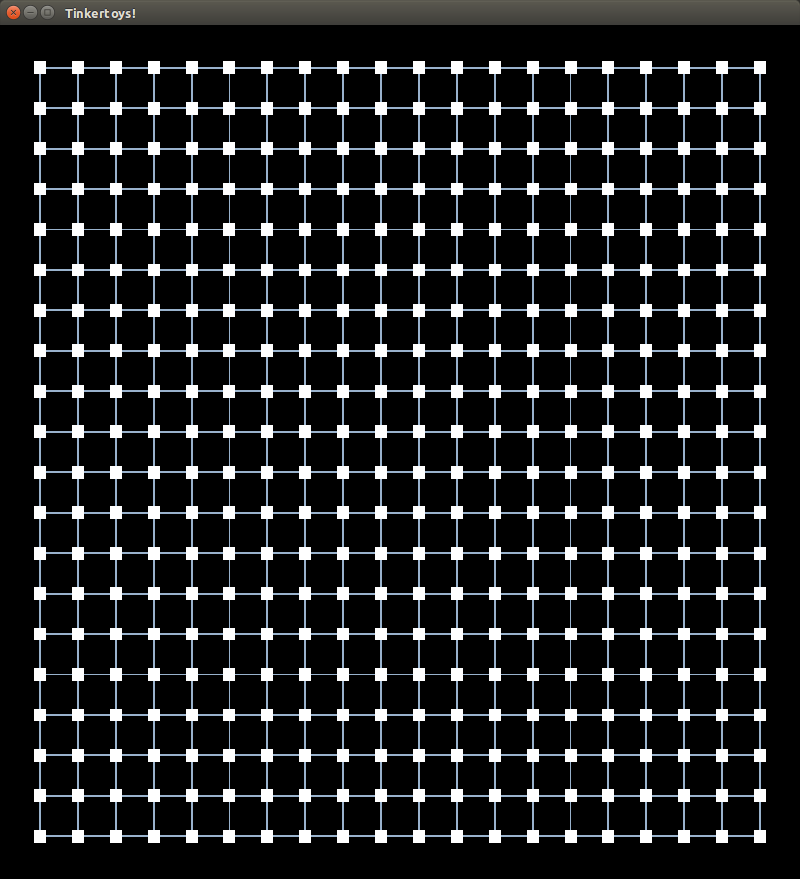
\includegraphics[width=\textwidth]{grid_start}
		\caption{Initial situation}
		\label{grid_start}
	\end{subfigure}
	~~
	\begin{subfigure}[b]{0.35\textwidth}
		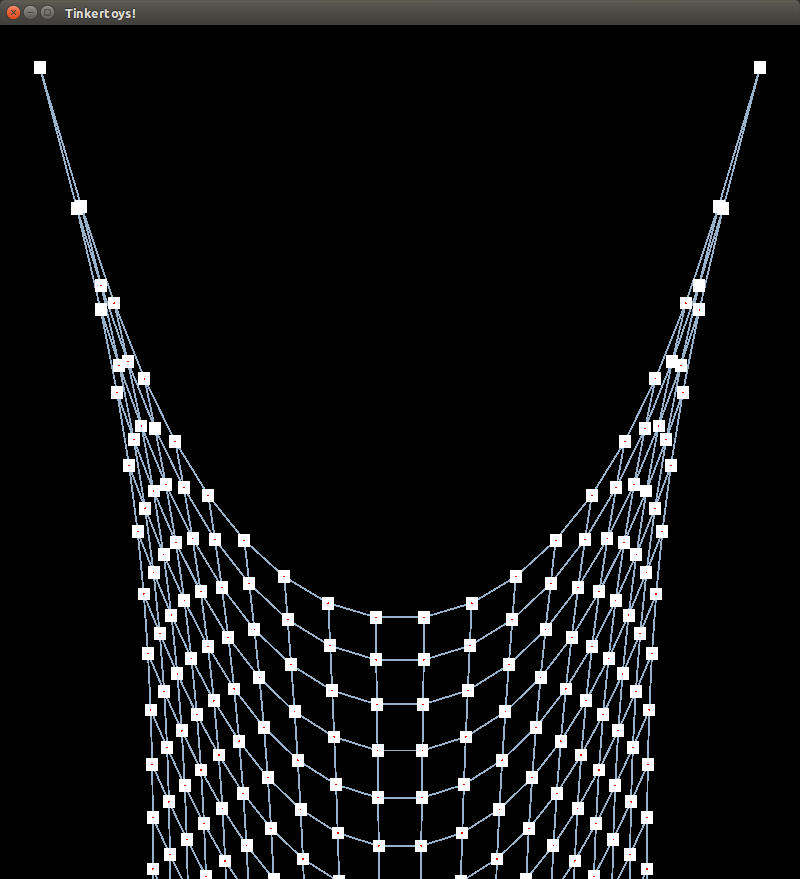
\includegraphics[width=\textwidth]{grid_rest}
		\caption{Stable situation}
		\label{grid_rest}
	\end{subfigure}
	\caption{Cloth without diagonal springs}
	\label{grid}
\end{figure*}
To simulate 2-dimensional cloth, we implemented a function that generates a square grid of particles, interconnected by springs in the x and y-directions. Optionally, diagonal springs can be added. The two upper particles are fixed in the upper corners of the screen. A grid without diagonal springs as seen in Figure~\ref{grid} behaves almost like cloth, with exception of shear forces, which make the grid collapse. This can be resolved by adding diagonal springs, which make the behavior of the cloth more natural. This is shown in Figure~\ref{diag}. One downside of this simple model is that it can get 'stuck' in a local minimum. This could be mitigated by adding connectivity between a particle with particles more at distance, outside of the direct neighbors.
The mass of the particles also affects the behavior of the cloth. When the mass is too big relative to the tension of the springs, the cloth stretches too much vertically to look realistic. When the springs are too string compared to the mass of the particles, the simulation becomes numerically instable.
\begin{figure*}[b]
	\centering
	\begin{subfigure}[b]{0.35\textwidth}
		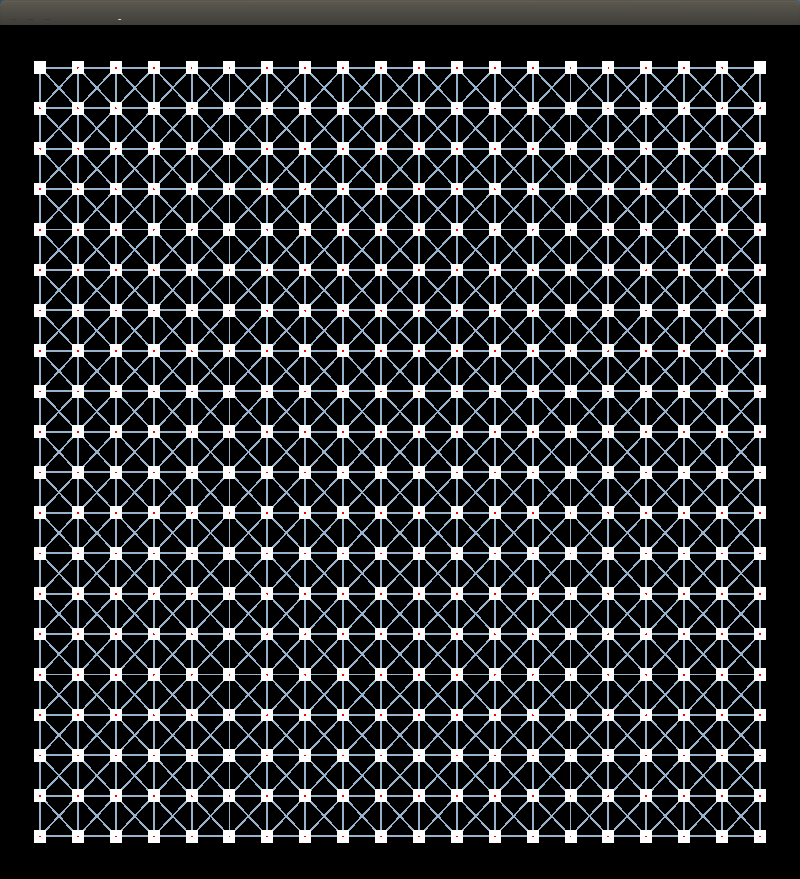
\includegraphics[width=\textwidth]{diag_start}
		\caption{Initial situation}
		\label{diag_start}
	\end{subfigure}
	~
	\begin{subfigure}[b]{0.35\textwidth}
		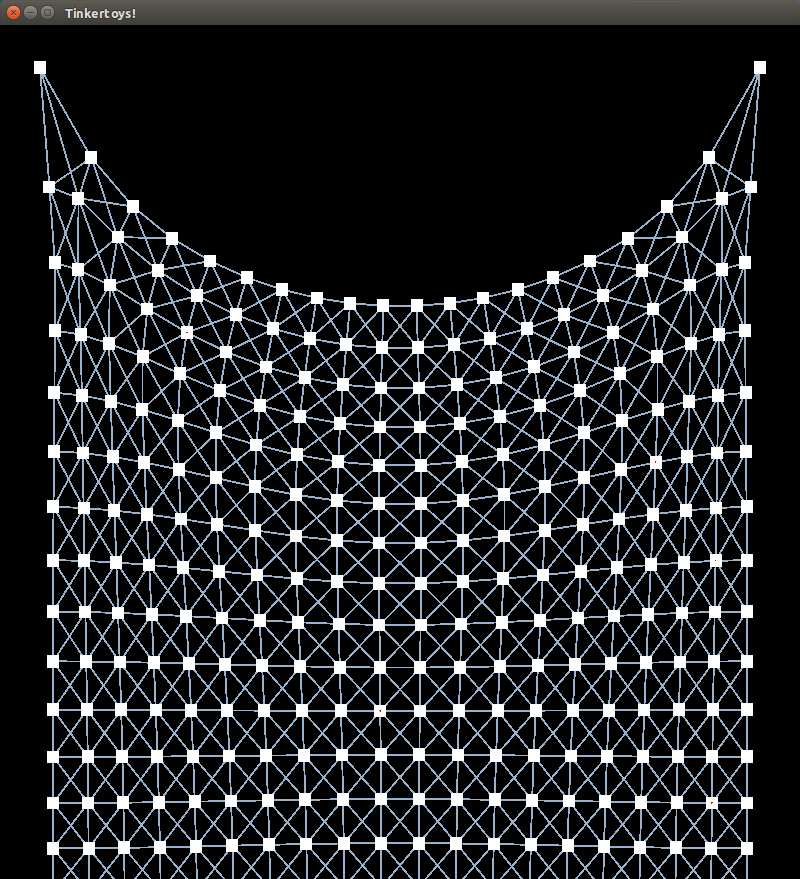
\includegraphics[width=\textwidth]{diag_rest}
		\caption{Stable situation}
		\label{diag_rest}
	\end{subfigure}
	\caption{Cloth without diagonal springs}
	\label{diag}
\end{figure*}
\begin{figure}[h]
	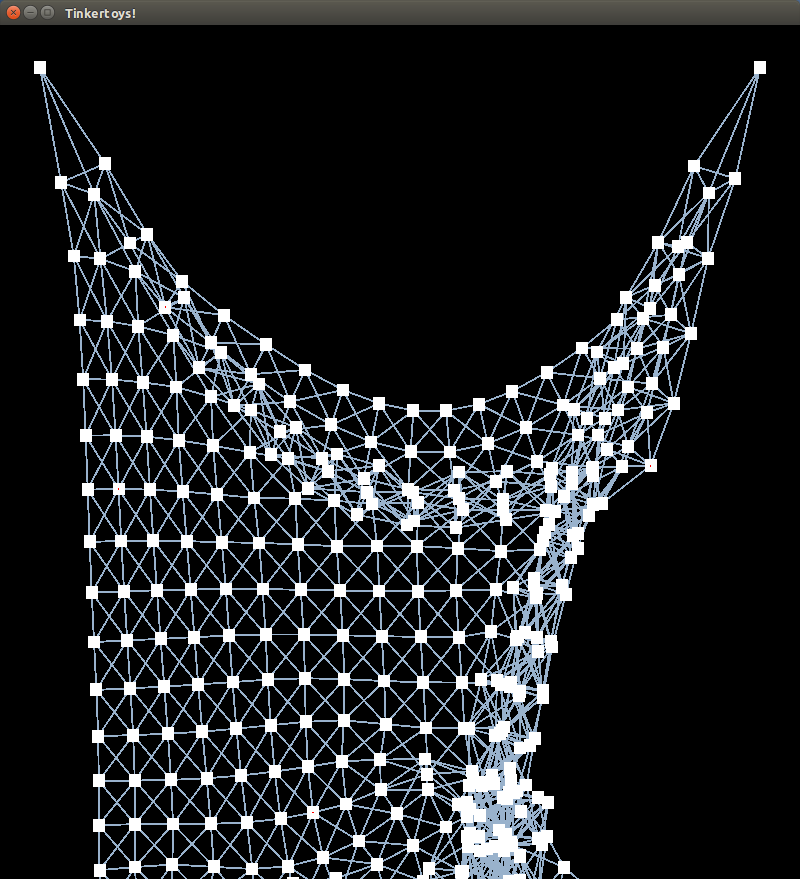
\includegraphics[width=0.4\textwidth]{diag_localmin}
	\caption{Cloth stuck in a local minimum}
	\label{diag_localmin}
\end{figure}
\end{document}
